\documentclass{article}
\usepackage{listings}
\usepackage{geometry}
\usepackage{amsmath,amsthm,amssymb}
\usepackage{hyperref}
\usepackage{color}
\usepackage{mathtools}
\usepackage[dvipsnames]{xcolor}
\usepackage{tikz-cd}

% mathbb shortcuts
\newcommand{\Z}{\mathbb{Z}}
\newcommand{\N}{\mathbb{N}}
\newcommand{\Q}{\mathbb{Q}}
\newcommand{\R}{\mathbb{R}}
\newcommand{\C}{\mathbb{C}}
\newcommand{\F}{\mathbb{F}}
\newcommand{\T}{\mathbb{T}}
\newcommand{\HH}{\mathbb{H}}
\newcommand{\RP}{\mathbb{RP}}
\newcommand{\PP}{\mathbb{P}}
\newcommand{\A}{\mathbb{A}}
\newcommand{\E}{\mathbb{E}}

% mathfrak shortcuts
\newcommand{\fI}{\mathfrak{I}}
\newcommand{\fA}{\mathfrak{A}}
\newcommand{\fG}{\mathfrak{G}}

% mathcal shortcuts
\newcommand{\cA}{\mathcal{A}}
\newcommand{\cU}{\mathcal{U}}
\newcommand{\cR}{\mathcal{R}}
\newcommand{\cP}{\mathcal{P}}
\newcommand{\cB}{\mathcal{B}}
\newcommand{\cC}{\mathcal{C}}
\newcommand{\cF}{\mathcal{F}}
\newcommand{\cS}{\mathcal{S}}

\newcommand{\Aut}{\textrm{Aut}}
\newcommand{\degg}{\textrm{deg}}
\newcommand{\Hom}{\textrm{Hom}}
\newcommand{\conj}{\textrm{conj}}
\newcommand{\Gal}{\textrm{Gal}}
\newcommand{\disc}{\textrm{disc}}
\newcommand{\supp}{\textrm{supp}}
\newcommand{\Jac}{\textrm{Jac}}
\newcommand{\Der}{\textrm{Der}}
\newcommand{\Spec}{\textsf{Spec}\,}
\newcommand{\im}{\textrm{im}\,}

% mathsf shortcuts
\newcommand{\Cell}{\textsf{Cell}}

\newcommand{\clr}{\color{red}}

\newtheorem{lemma}{Lemma}
\newtheorem{definition}{Definition}
\newtheorem{proposition}{Proposition}
\theoremstyle{definition}


\begin{document}

\begin{center}
	\large \textbf{GRST Notes:  0-1 Sheaves and Sam's Conjecture (February 3, 2017)} \\
\end{center}

This week, Brendan talked a bit about 0-1 sheaves, and discussed his implementation Sam's algorithm  described in the previous post. Additionally, Brendan shared a proof that for simplicial complexes, we only need to consider two layers at a time when we perform the random sheaf computations. As in previous blog posts, all sheaves are assumed to be valued in $\textsf{Vect}$.

\section{0-1 Sheaves}
A couple of seminar sessions ago, we discussed some easy examples of sheaf cohomology to try and figure out an intuitive way to think about the cohomology of simple sheaves. In the related blog post {\clr (link here)}, all of the examples were on 2-dimensional simplicial complexes where all stalks were one dimensional, and every map was either the identity map or the zero map. These are examples of 0-1 sheaves.

\begin{definition}
	Let $X$ be a simplicial complex. A \textbf{0-1 sheaf} on $X$ is a sheaf such that the stalk over each cell is $k$, and all restriction maps are either the zero map or the identity map.
\end{definition}

The reason we want to understand these sheaves is because they are simple, and hopefully by having an intuition about these 0-1 sheaves, we can build a better intuition about more complicated sheaves.  There are two main questions we have about these sheaves. Firstly, is there a way to classify all 0-1 sheaves on a given simplicial complex $X$. Secondly, is there an intuitive way to think about the first cohomology of such sheaves? In this post, we focus on the first problem.\\

One idea for classification is to relate all possible sheaves on $X$ to all possible partitions of its corresponding poset into convex subsets. Consider our favorite cell complex and its related poset.

\begin{figure}[!htbp]
\centering
	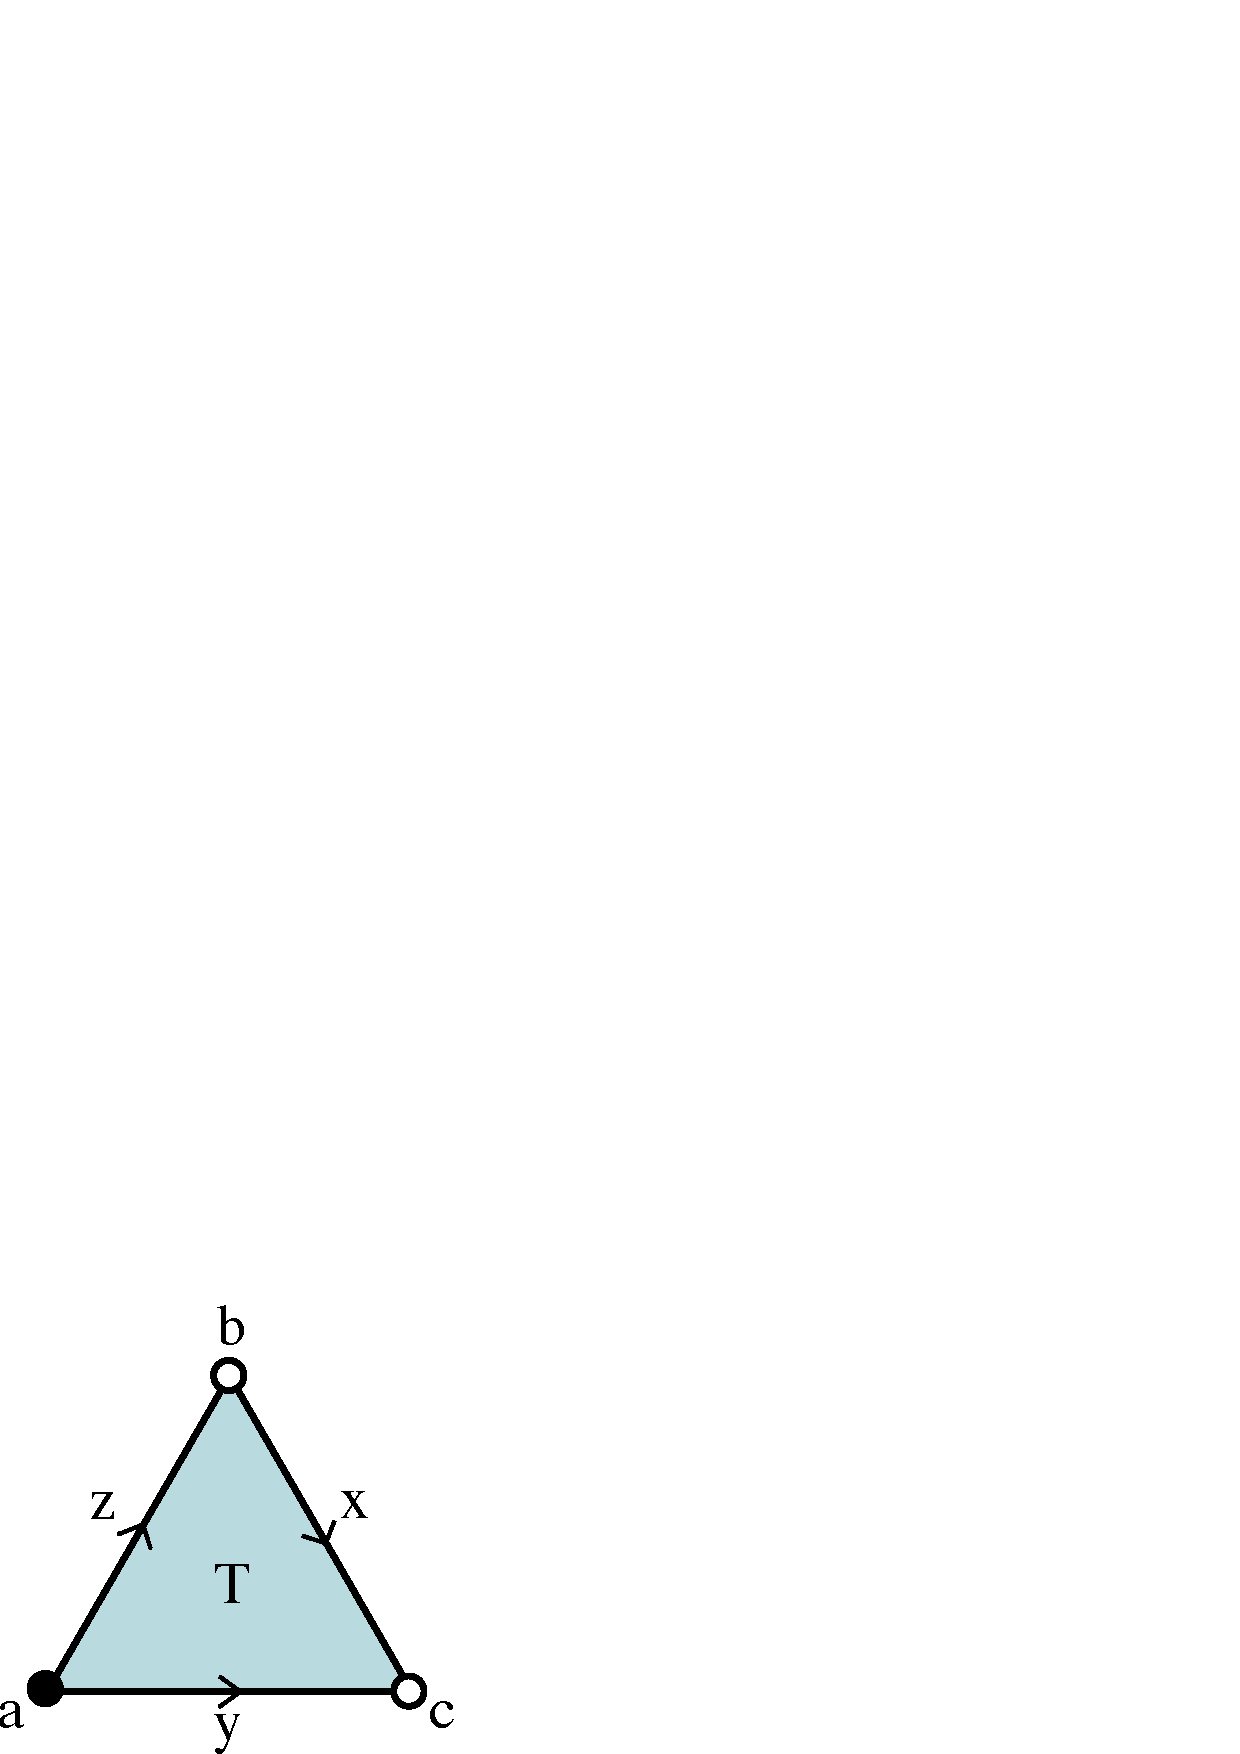
\includegraphics[width=0.2\textwidth]{images/triangle_dir.png}
\end{figure}

\[
\begin{tikzcd}
	& T & \\
	x \arrow{ur} & y \arrow{u} & z \arrow{ul} \\
	a \arrow{ur} \arrow{urr} & b\arrow{ur} \arrow{ul} & c \arrow{ul} \arrow{ull}
\end{tikzcd}
\]

For example, a partition of this poset into convex subsets is $\{a,y,z\}, \{b,c,x\}, \{T\}$. We keep all arrows that are inside a subset of the partition. Then, the poset breaks up as follows.
\[
\begin{tikzcd}
	& T & \\
	x \arrow[red]{ur} & y \arrow[red]{u} & z \arrow[red]{ul} \\
	a \arrow{ur} \arrow{urr} & b\arrow[red]{ur} \arrow{ul} & c \arrow[red]{ul} \arrow{ull}
\end{tikzcd}
 = 
 \begin{tikzcd}
	& T & \\
	{\color{white}x} \arrow[white]{ur} & {\color{white}y} \arrow[white]{u} & {\color{white}z} \arrow[white]{ul} \\
	{\color{white}a} \arrow[white]{ur} \arrow[white]{urr} & {\color{white}b}\arrow[white]{ur} \arrow[white]{ul} & {\color{white}c} \arrow[white]{ul} \arrow[white]{ull}
\end{tikzcd}
\oplus
\begin{tikzcd}
	& {\color{white}T} & \\
	x \arrow[white]{ur} & {\color{white}y} \arrow[white]{u} & {\color{white}z} \arrow[white]{ul} \\
	{\color{white}a} \arrow[white]{ur} \arrow[white]{urr} & b\arrow[white]{ur} \arrow{ul} & c \arrow[white]{ul} \arrow{ull}
\end{tikzcd}
\oplus
\begin{tikzcd}
	& {\color{white}T} & \\
	{\color{white}x} \arrow[white]{ur} & y \arrow[white]{u} & z \arrow[white]{ul} \\
	a \arrow{ur} \arrow{urr} & {\color{white}b}\arrow[white]{ur} \arrow[white]{ul} & {\color{white}c} \arrow[white]{ul} \arrow[white]{ull}
\end{tikzcd}
\]
where the red arrows on the left represent the arrows that point between two subsets in the partition. We define the 0-1 sheaf associated with this partition to have identity maps where the arrows are black, and zero maps where the arrows are red. Specifically, if an arrow lies inside a subset in the partition, it is an identity, and otherwise it is a zero map.\\

The restriction of the partition to convex subsets will ensure that this construction results in a sheaf. To check this, we need to make sure all commutativity relations hold between the maps that connect any two points $p_1$ and $p_2$ where $p_1 < p_2$. Suppose $p_1$ and $p_2$ are in the same subset. Then by convexity, any path of arrows that connect the two points are also in the same subset, and thus all maps from $p_1$ to $p_2$ will be the identity map. Suppose $p_1$ and $p_2$ are in different subsets. This means that every path of arrows from $p_1$ to $p_2$ will include a zero map. Suppose not, and that there exists a path of identity maps from $p_1$ to $p_2$. Then there must be a path connecting $p_1$ and $p_2$, contradicting the fact that they should be in different subsets.\\

However, we note that not all 0-1 sheaves can be constructed in this manner. Consider the triangle without the $2$-cell filled in, and consider the following 0-1 sheaf.
\[
\begin{tikzcd}
	x & y & z \\
	a \arrow[red]{ur} \arrow{urr} & b\arrow{ur} \arrow{ul} & c \arrow{ul} \arrow{ull}
\end{tikzcd}
\]
We note that this is indeed a sheaf. Suppose this were constructed using the partitioning method so that $a$ must be disconnected from $y$. Then, since both $a$ and $b$ are connected to $z$, $a$ and $b$ must be in the same subset. Similarly, since both $b$ and $c$ are connected to $x$, $b$ and $c$ are in the same subset. Therefore, $a$ and $c$ are in the same subset, but $c$ is connected to $y$, which is a contradiction. \\

Therefore, this shows that every partition of the poset into convex subsets gives a 0-1 sheaf, but not necessarily the other way around. Does there exist a condition that allows us to classify all 0-1 sheaves?

\section{Sam's Conjecture}
Now, we move away from 0-1 sheaves and consider the top-down construction of a random sheaf described in the last post. Recall that at each step of the algorithm, we take the limit of the reduced open star of a given star in the diagram. When we are working with large and high dimensional cell complexes, this diagram can become quite large. It woud be interesting to see if we can work with a smaller diagram but still get the same result. Brendan came up with a proof where we can reduce the diagram for a simplicial complex.

\begin{proposition}
Suppose $X$ is a Liorian over a simplicial complex, and $F$ is the sheaf over $X$ that we are constructing. Suppose all maps out of simplexes with dimension greater than $k$ have been defined (according to the algorithm). Let $\sigma$ be a $k$ cell, and $\mathrm{star}(\sigma)$ be its reduced open star. Denote $\mathrm{star}^{k+2}(\sigma) = \mathrm{star}(\sigma) \cap X^{k+2}$, where $X^k$ is the $k$-skeleton of $X$.  Then, we have
\begin{equation}
	\lim_{\longleftarrow} F(\mathrm{star}(\sigma)) = \lim_{\longleftarrow} F(\mathrm{star^{k+2}}(\sigma)).
\end{equation}
\end{proposition}
Pictorially, this means that we only have to look at the two dimensions above any cell $\sigma$.

\[
\begin{tikzcd}
	\vdots & \vdots & \vdots \\
	x \arrow[dashed]{ur} \arrow[dashed]{u}& y \arrow[dashed]{u} & z \arrow[dashed]{u} \arrow[dashed]{ul}\\
	a \arrow{ur} \arrow{urr} & b\arrow{ur} \arrow{ul} & c \arrow{ul} \arrow{ull} \\
	& L \arrow{ul} \arrow{u} \arrow{ur} &
\end{tikzcd}
\hspace{15pt}=\hspace{15pt}
\begin{tikzcd}
	{\color{white}\vdots} & {\color{white}\vdots} & {\color{white}\vdots} \\
	x & y & z \\
	a \arrow{ur} \arrow{urr} & b\arrow{ur} \arrow{ul} & c \arrow{ul} \arrow{ull} \\
	& L \arrow{ul} \arrow{u} \arrow{ur} &
\end{tikzcd}
\]

\begin{proof}
We claim that there exists a bijection between the two sets.
\begin{equation}
	\{\textrm{cones over} \, F(\mathrm{star}(\sigma))\} = \{\textrm{cones over} \, F(\mathrm{star}^{k+2}(\sigma))\}
\end{equation}
Given a cone over $F(\mathrm{star}(\sigma))$, it is clear that the restriction of this cone to $X^{k+2}$ is a cone over $F(\mathrm{star}^{k+2}(\sigma))$. \\

Alternatively, suppose we have a cone over $F(\mathrm{star}^{k+2}(\sigma))$ with vertex $C$ and we are trying to extend it to a cone over $F(\mathrm{star}(\sigma))$. Let $\tau$ be an element of $\mathrm{star}(\sigma)$ that is not in $X^{k+2}$ so that maps into $\tau$ are not a priori defined. We claim that the map $C \rightarrow \tau$ is well defined by the maps in $\mathrm{star}^{k+2}(\sigma)$. Indeed, suppose $a,b \in \tau$, so that $\sigma\cup a$ and $\sigma \cup b$ are $(k+1)$-simplexes that are faces of $\tau$. Note that we are writing simplexes as a set of vertices. Then, the following diagram commutes.
\[
\begin{tikzcd}
 & \sigma \cup \{a\} \arrow{dr} \arrow[bend left=20]{drr} & & \\
 \sigma \arrow{ur} \arrow{dr} & & \sigma\cup\{a,b\} \arrow{r} & \tau \\
 & \sigma \cup \{b\} \arrow{ur} \arrow[bend right=20]{urr} & &
\end{tikzcd}
\]
where all of the maps into $\tau$ are well defined since all maps out of simplexes with dimension larger than $k$ have been defined according to the algorithm. Note that the existence of $\sigma \cup \{a,b\}$ exists as a face because this is a simplicial complex. This ensures the commutativity of the diagram. Therefore, a cone over $F(\mathrm{star}^{k+2}(\sigma))$ extends uniquely to the full reduced open star.

\end{proof}

\end{document}